\documentclass{sig-alternate-ipsn13}

\usepackage{graphicx}
\DeclareGraphicsExtensions{.pdf,.png,.jpg}
\graphicspath{ {img/} }

\newcommand\T{\rule{0pt}{2.6ex}}
\newcommand\B{\rule[-1.2ex]{0pt}{0pt}}

%---------------------------------------------------------------------%
\begin{document}

%---------------------------------------------------------------------%
\title{On Developing User Interfaces for Piloting Unmanned Systems}
\author{James Edmondson ~~~~~~ Gene Cahill ~~~~~~ Anthony Rowe\\
Carnegie Mellon University, Pittsburgh, USA \\
\email{\{jredmondson,gene.cahill\}@sei.cmu.edu, agr@ece.cmu.edu}}
%---------------------------------------------------------------------%
\maketitle

%---------------------------------------------------------------------%
\begin{abstract}
Current artificial intelligence (AI) control paradigms tend to be one-to-one in
nature and cater to
monolithic systems, e.g., between one operator and one large, multi-functional
robot. However, the future of AI is likely to be smaller, more distributed, and
larger scale. Along that path, major advances have been made in the
commercialization of smaller unmanned autonomous systems (UAS) like
quad-copters and small ground-based robots that are equipped with wireless
radios for communication between these systems and human operators, control
stations, or other UAS. Even for systems built with capabilities for
communication between UAS, the main control paradigm for such systems largely
remains the same one-to-one paradigm and is geared toward joystick control or
waypoint-based systems that force operators to define the complete paths for
each UAS participating in a mission environment.

In this paper, we will discuss recent efforts in user interface (UI) design in
the Group Autonomy for Mobile Systems project at Carnegie Mellon University.
The goal of the UI development is to reduce the cognitive load forced on human
operators, especially those wanting to use swarms of devices in mission-critical
contexts like search-and-rescue.  We detail the coupling of distributed AI
algorithms with these map-based, minimalistic interfaces, and highlight the
decreased required user actions to accomplish similar swarm-based maneuvers
against waypoint-based guidance systems. We believe these types of interfaces
may prove pivotal in bringing group-based UAS control into more mainstream usage.

\end{abstract}

%---------------------------------------------------------------------%
\section{introduction}

As unmanned aerial vehicles and ground robots become less expensive and more
pervasive, the need for intuitive control interfaces for multiple distributed
systems in environments such as search-and-rescue, resource exploration, and
other situations becomes more pronounced. However, current generations of
interfaces for controlling multiple unmanned systems focus on micro-manipulation
of individual systems within a swarm of autonomous entities. For instance, an
interface for such a grouping of systems may require an operator to select one
or more entities and give them a proximate waypoint, often via GPS, to move to.
Examples of existing systems that do this include the AR.Drone 2.0 Free Flight
Flight Recorder Application~\cite{irizarry2012usability};
the 3D Robotics Mission Planner, Droid Planner,
APM Planner~\cite{arora2013development}; and AFRL's ATAK mission
planning environment~\cite{gillen2012beyond}.
These concepts are extended further in 3D piloting systems based on landmark
navigation~\cite{ranft20133d} and augmented reality~\cite{kochflying}, as
these interfaces tend to require the full attention
of an operator on each UAS, rather than focusing on the group operations.

This type of system is cumbersome as the group size becomes larger and the
state-of-the-art trends toward control paradigms of one human operator, often
with a hand held controller, to one robotic system. This has hampered the
adoption of multi-robot systems by agencies and companies that could highly
benefit from the usage of multi-robot systems, such as search-and-rescue crews,
because a high training cost is associated with multi-robot systems, due to each
robot system requiring its own pilot. To reduce the cognitive load required in
multi-robot system navigation and usage, we believe that user interfaces should
be combined with distributed artificial intelligence underneath the UI and
within the robotic systems to all single operators to more readily control
multiple unmanned systems.

In this paper, we describe work done in the Group Autonomy for Mobile Systems
(GAMS) project at Carnegie Mellon University that focuses on interfaces and
tightly coupled distributed artificial intelligence algorithms that enable a single
operator to control multiple unmanned systems. We highlight developed interfaces
that effect area coverage with thermal sensors and also network bridging to
connect operators across multi-hop communication paths using a small swarm of
unmanned aerial vehicles.


%---------------------------------------------------------------------%
\section{The Problem with the State-of-the-Art}
\label{sec:waypoints}

\begin{figure}[htb]
  \centering
  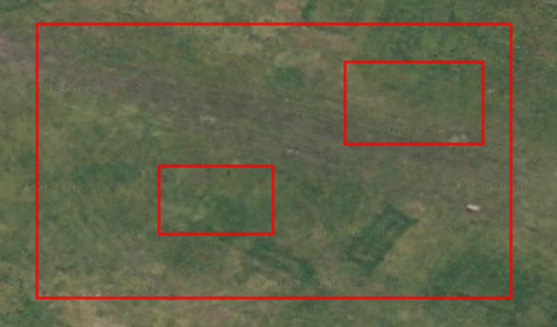
\includegraphics[scale=0.4]{guiding_scenario}
  \caption{Mission Scenario Provided to Three Untrained Users}
  \label{fig:guiding}
\end{figure}

To understand the benefits of the GAMS interfaces, we must first explore some
of the problems with the state-of-the-art. In this section, we describe some
simple, repeatable experiments with waypoint navigation systems, which as
mentioned in Section~\ref{sec:introduction} are
used in software like AR.Drone 2.0 Free Flight
Flight Recorder Application~\cite{irizarry2012usability};
the 3D Robotics Mission Planner, Droid Planner,
APM Planner~\cite{arora2013development}; and AFRL's ATAK mission planning
environment~\cite{gillen2012beyond}.


\begin{figure}[h]
  \centering
  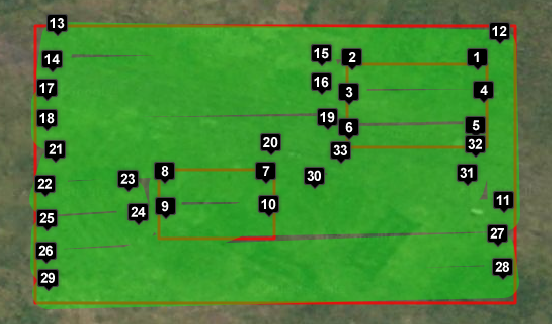
\includegraphics[scale=0.4]{user_waypoints_1}
  \caption{User 1 First Plot}
  \label{fig:user1_1}
\end{figure}

\begin{figure}[h]
  \centering
  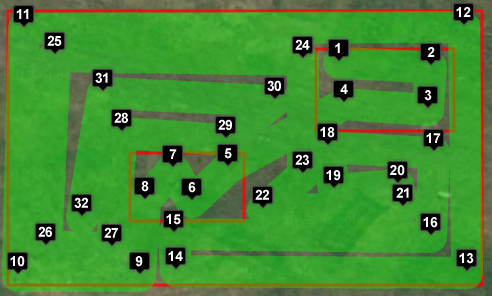
\includegraphics[scale=0.4]{user_waypoints_2}
  \caption{User 1 Second Plot}
  \label{fig:user1_2}
\end{figure}


In a waypoint navigation system, the user must select a device in an interface
and then select a waypoint to traverse to. Most of these interfaces allow users
to queue up waypoints (essentially plot a path of points), which allows an
operator to plan out complicated missions. Figure ~\ref{fig:guiding} lays out
the mission we asked of three volunteers, whom we allowed to replot their
missions after seeing results that displayed the required clicks and the area
that actually ended up being covered. The larger area is the main search area
and the smaller areas are priority regions, places that are more important due
to the mission and must be searched quickly (e.g., in a search-and-rescue
mission where known survivors are at and triage decisions need to be made).

\iffalse

\begin{figure}[h]
  \centering
  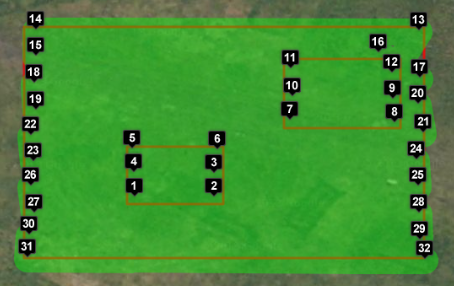
\includegraphics[scale=0.45]{user_waypoints_3}
  \caption{User 2 First  Plot}
  \label{fig:user2_1}
\end{figure}

\fi

\begin{figure}[h]
  \centering
  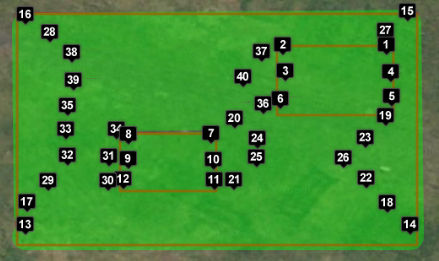
\includegraphics[scale=0.5]{user_waypoints_4}
  \caption{User 2 Second Plot}
  \label{fig:user2_2}
\end{figure}

The following figures (Figure ~\ref{fig:user1_1}, 
~\ref{fig:user2_2}, ~\ref{fig:user3_2})
are the results of handing the waypoint navigation to random
people in our research lab, one of whom had experience flying waypoint systems.
For space reasons, we picked only the three that showed the most interesting
characters--whether showing higher user error or excessive diligence.

These are by no means meant to categorically and exhaustively explore the space
of user interactions possible in the system. We show these here to highlight the
differences between the mission requirements and the kinds of errors that are likely with
human usage. Additionally, after these images, we breakdown the average user
actions required to send one drone on a mission like this. As swarms grow larger,
the waypoint system becomes even more cumbersome to use.

\iffalse
\begin{figure}[h]
  \centering
  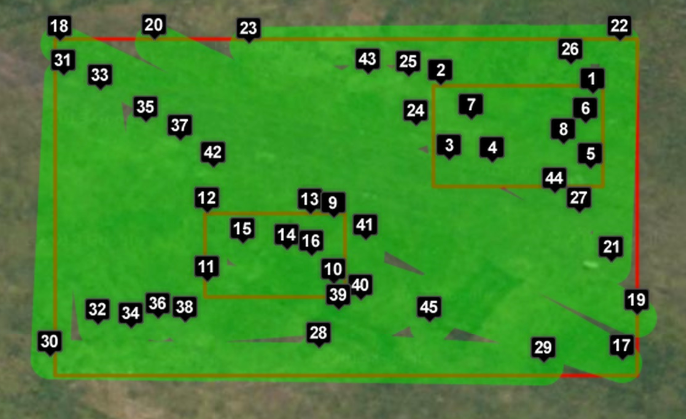
\includegraphics[scale=0.3]{user_waypoints_5}
  \caption{User 3 First  Plot}
  \label{fig:user3_1}
\end{figure}
\fi

\begin{figure}[h]
  \centering
  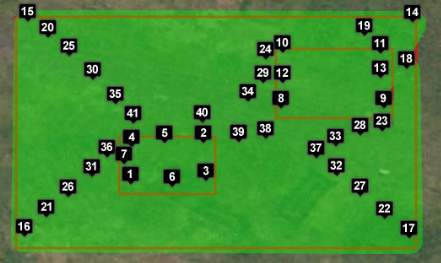
\includegraphics[scale=0.45]{user_waypoints_6}
  \caption{User 3 Second Plot}
  \label{fig:user3_2}
\end{figure}

Table ~\ref{tab:averagewaypoints} shows the marker counts, readjustments,
user actions and time taken to use the waypoint navigation interface to search these
three areas. The time taken and user actions varied wildly, and the accuracy of the
search was also highly variable. These results highlight some of the problems in
using such waypoint-based systems in mission-critical contexts like
search-and-rescue but also in agriculture or any number of other scenarios where
accuracy is important. A
UAV attempting to spray pesticides over a field and missing large patches can
be disasterous for crop growth and maintenance. A UAV that does not locate a
survivor could result in unnecessary fatalities and improper triage in a disaster
area. 

\begin{table}[htb]
\caption{Results of Waypoint Navigation System Usage}
\label{tab:averagewaypoints}
\centering
\begin{tabular}{|l|l|l|l|}
\hline

Observable \T & Min & Max & Avg \\
\hline Marker Count \T & 32 & 45 & 37.166 \\ 
Readjusts & 0 & 31 & 9.166 \\ 
User Actions & 32 & 71 & 46.333 \\ 
Time Taken \B & 51s  & 123s & 79.706s \\ \hline
\end{tabular}
\end{table}

In the next section, we will discuss the results of using the GAMS
interface on similar problems. 

%---------------------------------------------------------------------%
\section{The GAMS Interface and Software}
\label{sec:gams_interface}

As we have shown in section ~\ref{sec:waypoints}, waypoint-based
navigation systems are highly error prone and take a significant amount
of time to task UAVs in even small mission contexts. In this section, we
outline changes we have made to a map-based interface to facilitate
mission-focused UAV tasking that requires less user actions and time,
making it more suitable, especially, for high cognitive load situations like
search-and-rescue.

The usage of the GAMS interface includes the following steps:
\begin{enumerate}
  \item Select the UAS that will be participating with a box or by list of names
  \item Select an action to perform from a list
  \begin{enumerate}
    \item Primitive operations
    \item Network bridging between two locations
    \item Area coverage
    \item Priority area coverage
  \end{enumerate}
\end{enumerate}

Primitive operations are functions like takeoff, land, move-to-gps, and other
operations that are considered primitive AI. Network bridging is an instruction
to the drones to move to locations that allow network traffic to pass between
locations. Area coverage is a distributed AI that causes the drones to collaborate
to cover a single rectangular area. Prioritized area coverage is a distributed AI
that allows for the designation of prioritized regions within a main area coverage
that the UAS will try to cover first.

The underlying artificial intelligence is implemented in the MADARA Knowledge and
Reasoning Engine (KaRL) engine ~\cite{Edmondson-KaRL-ksem2011}, a specialized
and fast, real-time reasoning engine that was built for contextual inferencing in
distributed, decentralized sensor networks. Our interface, which allows
interaction with this AI, is built in Java for any device running the Android
operating system. This allows us to control a swarm from a tablet or smartphone.
Both the interfaces and the AI is released as open source under a BSD license
at http://gams-cmu.googlecode.com.

In the next section, we will detail a small series of experiments that showcase the
power of the interface and how it improves on the state-of-the-art in both required
user actions and time taken to input a new swarm mission.

%---------------------------------------------------------------------%
\section{Experimental Results}
\label{sec:exp}

\begin{table}[ht]
\caption{Comparison of GAMS and Waypoint Interface}
\label{tab:expresults}
\centering
\begin{tabular}{|l|l|l|l|l|l|}
\hline

Interface \T & $\gamma$ & $\beta$ & $\delta$ & $\kappa$ & $\rho$ \\
\iffalse 
\hline 1 & GAMS \T & 3 & 20 & N/A & 100 & 0 \\ 
1 & GAMS & 3 & 40 & N/A & 100 & 0 \\ 
1 & GAMS \B & 3 & 80 & N/A & 100 & 0 \\ 
\hline 1 & Waypoints \T & 11 & 20 & 0 & 100 & 0 \\ 
1 & Waypoints & 21 & 40 & 0 & 100 & 0 \\ 
1 & Waypoints \B & 41 & 80 & 0 & 100 & 0 \\
\fi

\hline GAMS \T & 4 & 20 & N/A & 1.0 & 0 \\ 
GAMS & 4 & 40 & N/A & 1.0 & 0 \\ 
GAMS \B & 4 & 80 & N/A & 1.0 & 0 \\  \hline
Waypoints \T & 12 & 20 & 0 & 1.0 & 0 \\ 
Waypoints & 22 & 40 & 0 & 1.0 & 0 \\ 
Waypoints \B & 42 & 80 & 0 & 1.0 & 0 \\ \hline
Waypoints \T& 9 & 20 & -0.4 & 0.6 & 0 \\ 
Waypoints & 16 & 40 & -0.4 & 0.6 & 0 \\ 
Waypoints \B & 31 & 80 & -0.4 & 0.6 & 0 \\ \hline
Waypoints \T& 10 & 20 & -0.2 & 0.8 & 0 \\ 
Waypoints & 19 & 40 & -0.2 & 0.8 & 0 \\ 
Waypoints \B & 35 & 80 & -0.2 & 0.8 & 0 \\ \hline
Waypoints \T& 15 & 20 & 0.2 & 1.0 & 0.2 \\ 
Waypoints & 27 & 40 & 0.2 & 1.0 & 0.2 \\ 
Waypoints \B & 52 & 80 & 0.2 & 1.0 & 0.2 \\ \hline
Waypoints \T& 19 & 20 & 0.4 & 1.0 & 0.4 \\ 
Waypoints & 35 & 40 & 0.4 & 1.0 & 0.4 \\ 
Waypoints \B & 69 & 80 & 0.4 & 1.0 & 0.4 \\ \hline
\end{tabular}
\end{table}

Table~\ref{tab:expresults} details the results of comparing the optimal usage of
a waypoint system and the GAMS interface to perform area coverage with
two UAS ($n=2$) with a 4 meter sensor radius ($\theta$). Due to space limitations and
symmetry between number of drones used and minimum actions required, we
only show the usage of two drones. The table reflects the following
mathematical equation for determining user actions from a waypoint system.
%
\[
\gamma = 2 \left (\frac {\beta} {\theta (1 - \delta)} \right) + n
\]
%
Where $\beta$ is the length of the shortest side of a rectangular search area.
This is the key metric for determining the minimum number of waypoints required
by a waypoint interface
because of how it interacts with $\theta$, the sensor radius of the UAS. $\gamma$ is
the minimum number of user actions required and is what we attempt to minimize in this
research. $\delta$ is
the user error as an underestimate or overestimate of the sensor radius by the
human operator. $\kappa$ represents the percentage of area covered as a result
of the user actions. This becomes more important as results are shown when the
user has deviations in $\delta$ (the user error in approximating sensor radius).
$\rho$ represents the percentage of overlap, which happens when the user
underestimates $\theta$ and is indicated as a positive $\delta$.
Finally,
$n$ is the number of UAS, which is set to 2 due to space reasons and not shown in table.

The major takeaways from this data are that the waypoint system interface, even
with just two drones, requires more user actions than the GAMS interface.
Additionally, as shown in Section~\ref{sec:waypoints}, waypoint systems are prone to
error, and the more error inserted into guessing the sensor radius, the more actions
required and the more the area covered has overlaps or gaps. In the expressed data,
we do not require additional user actions ($\gamma$) to fix gaps in the area covered
by waypoint navigation systems.


%---------------------------------------------------------------------%
\section{Future Work and Conclusion}
\label{sec:conc}

In this paper, we have discussed insights into research conducted in the Group
Autonomy for Mobile Systems project at Carnegie Mellon University in regards
to user interfaces for swarms of unmanned autonomous systems. The user
interfaces developed and showcased here have been shown to decrease
user actions required and also reduce error by relying on autonomy within
the devices to cover areas correctly. Future work on this project is directed toward
using these interfaces to direct dozens of UAS to perform complex mission tasks
for search-and-rescue, agriculture, border patrol, and other tasks.

All interfaces and code are available as open source at
http://gams-cmu.googlecode.com.

%---------------------------------------------------------------------%
\section{Acknowledgements}
\label{sec:acknowledgements}

This material is based upon work funded and supported by the Department of
Defense under Contract No. FA8721-05-C-0003 with Carnegie Mellon University
for the operation of the Software Engineering Institute, a federally funded research
and development center. This material has been approved for public release and
unlimited distribution. Carnegie Mellon is registered in the U.S. Patent and
Trademark Office by Carnegie Mellon University. DM-0001018

%---------------------------------------------------------------------%
\bibliographystyle{abbrv} \bibliography{gams}

%---------------------------------------------------------------------%
\end{document}
